% asset_id: OffSpecNumericalMethodsTikZ-002
% source: AI-proposed printable reconstruction of midpoint diagram from supplied evidence
% status: Off-spec enrichment, not CCEA Further Mathematics core
\documentclass[tikz,border=8pt]{standalone}
\usepackage{amsmath}\usetikzlibrary{arrows.meta,calc}
\definecolor{Canvas}{HTML}{FAF9F6}\definecolor{Ivory}{HTML}{FFFFF0}\definecolor{LineGrey}{HTML}{E5E5EA}\definecolor{AccentGold}{HTML}{C5A059}\definecolor{SoftPink}{HTML}{FBEFEF}\definecolor{TextMath}{HTML}{2C2C2E}\definecolor{Predicted}{HTML}{D94F70}\definecolor{Actual}{HTML}{7FB069}\definecolor{PointBlue}{HTML}{3D5A80}
\begin{document}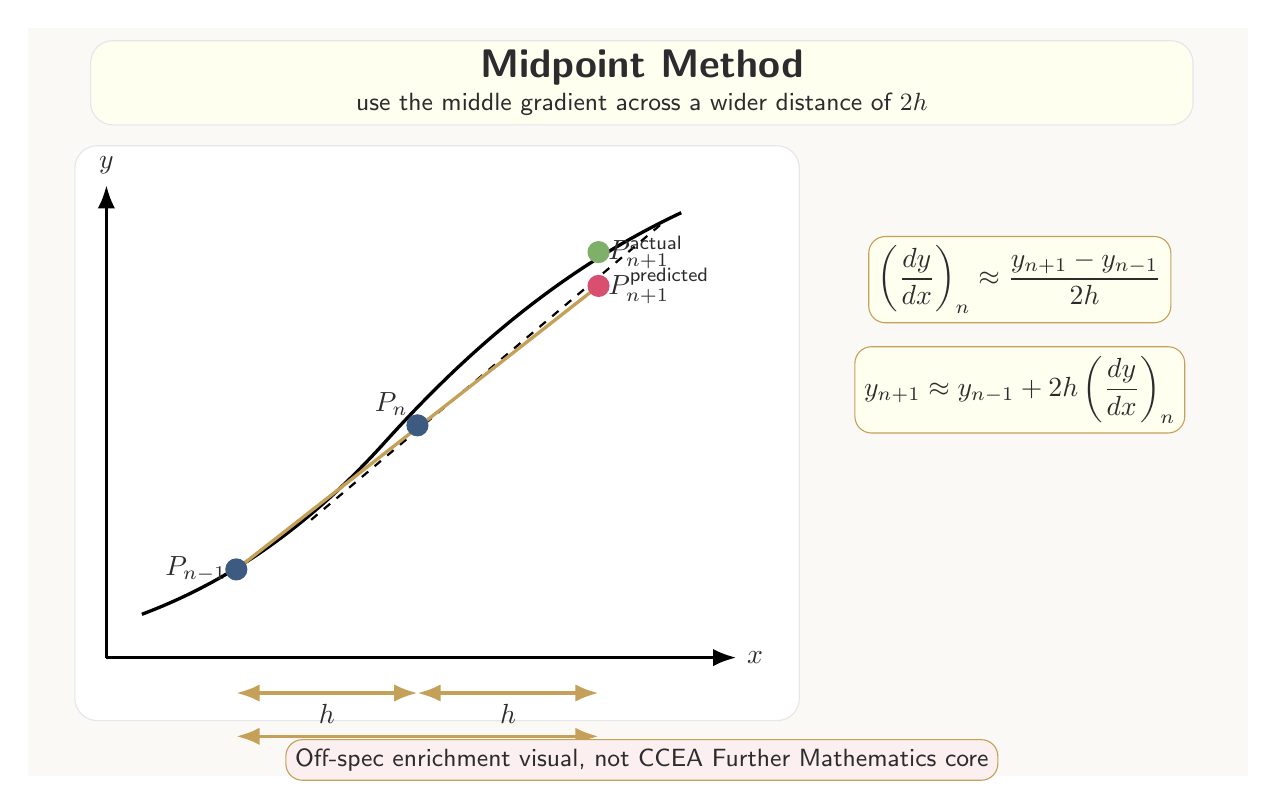
\begin{tikzpicture}[>=Latex,every node/.style={font=\sffamily,text=TextMath}]
\fill[Canvas](-1,-1.5)rectangle(14.5,8);\node[draw=LineGrey,fill=Ivory,rounded corners=8pt,minimum width=14cm,minimum height=1cm,align=center]at(6.8,7.3){\Large\textbf{Midpoint Method}\\\small use the middle gradient across a wider distance of $2h$};
\draw[draw=LineGrey,fill=white,rounded corners=8pt](-.4,-.8)rectangle(8.8,6.5);\draw[->,very thick](0,0)--(8,0)node[right]{$x$};\draw[->,very thick](0,0)--(0,6)node[above]{$y$};
\draw[very thick](.45,.55)..controls(1.65,1)and(2.65,1.75)..(3.55,2.75)..controls(4.5,3.8)and(5.7,4.9)..(7.3,5.65);
\coordinate(Pm)at(1.65,1.12);\coordinate(Pn)at(3.95,2.95);\coordinate(Pa)at(6.25,5.15);\coordinate(Pp)at(6.25,4.72);
\draw[dashed,thick](2.6,1.75)--(7.1,5.55);\draw[very thick,AccentGold](Pm)--(Pp);\fill[PointBlue](Pm)circle(4pt);\fill[PointBlue](Pn)circle(4pt);\fill[Actual](Pa)circle(4pt);\fill[Predicted](Pp)circle(4pt);
\node[left]at(Pm){$P_{n-1}$};\node[above left]at(Pn){$P_n$};\node[right]at(Pa){$P_{n+1}^{\text{actual}}$};\node[right]at(Pp){$P_{n+1}^{\text{predicted}}$};
\draw[<->,very thick,AccentGold](1.65,-.45)--(3.95,-.45)node[midway,below]{$h$};\draw[<->,very thick,AccentGold](3.95,-.45)--(6.25,-.45)node[midway,below]{$h$};\draw[<->,very thick,AccentGold](1.65,-1)--(6.25,-1)node[midway,below]{$2h$};
\node[draw=AccentGold,fill=Ivory,rounded corners=6pt,align=center]at(11.6,4.8){$\displaystyle \left(\frac{dy}{dx}\right)_n\approx\frac{y_{n+1}-y_{n-1}}{2h}$};\node[draw=AccentGold,fill=Ivory,rounded corners=6pt,align=center]at(11.6,3.4){$\displaystyle y_{n+1}\approx y_{n-1}+2h\left(\frac{dy}{dx}\right)_n$};
\node[draw=AccentGold,fill=SoftPink,rounded corners=6pt,align=center] at (6.8,-1.3){\small Off-spec enrichment visual, not CCEA Further Mathematics core};
\end{tikzpicture}\end{document}
